\newpage
\chapter{Architecture}
%Her beskrives den overordnede systemarkitektur vha. en domænemodel efterfulgt af SysML/UML. Der tages stilling til hvilke dele af projektet, der skal realiseres i HW og hvilke der skal realiseres vha. SW. De vigtigste dele af arkitekturen beskrives for systemets HW og SW i en sådan grad, at læseren får det fornødne overblik over systemet. Der fokuseres på opdeling i blokke, moduler, pakker, klasser etc. Der fokuseres ligeledes på hvordan disse blokke/moduler/pakker/klasser kommunikerer indbyrdes, dvs. de overordnede signaler/protokoller beskrives. For beskrivelse af detaljer angives reference til jeres ”arkitekturdokument” i projektets bilag.

In this section the hardware and software architecture will be discussed. The architecture is the ground work that enables the design of the system. Taking the requirements and dividing it in to blocks, modules, etc.

For a more in depth explanations of the different subjects discussed in this section, one can have a look at the \nameref{sec:sys-architecture}, section~\ref{sec:sys-architecture}, on page~\pageref{sec:sys-architecture} in the documentation.

\section{Hardware architecture}
To get a better understanding of the components what are need for this system. A block definition diagram or BDD was devised, as seen on figure~\ref{fig:generalbdd}. 

\begin{figure}[H]
\centering
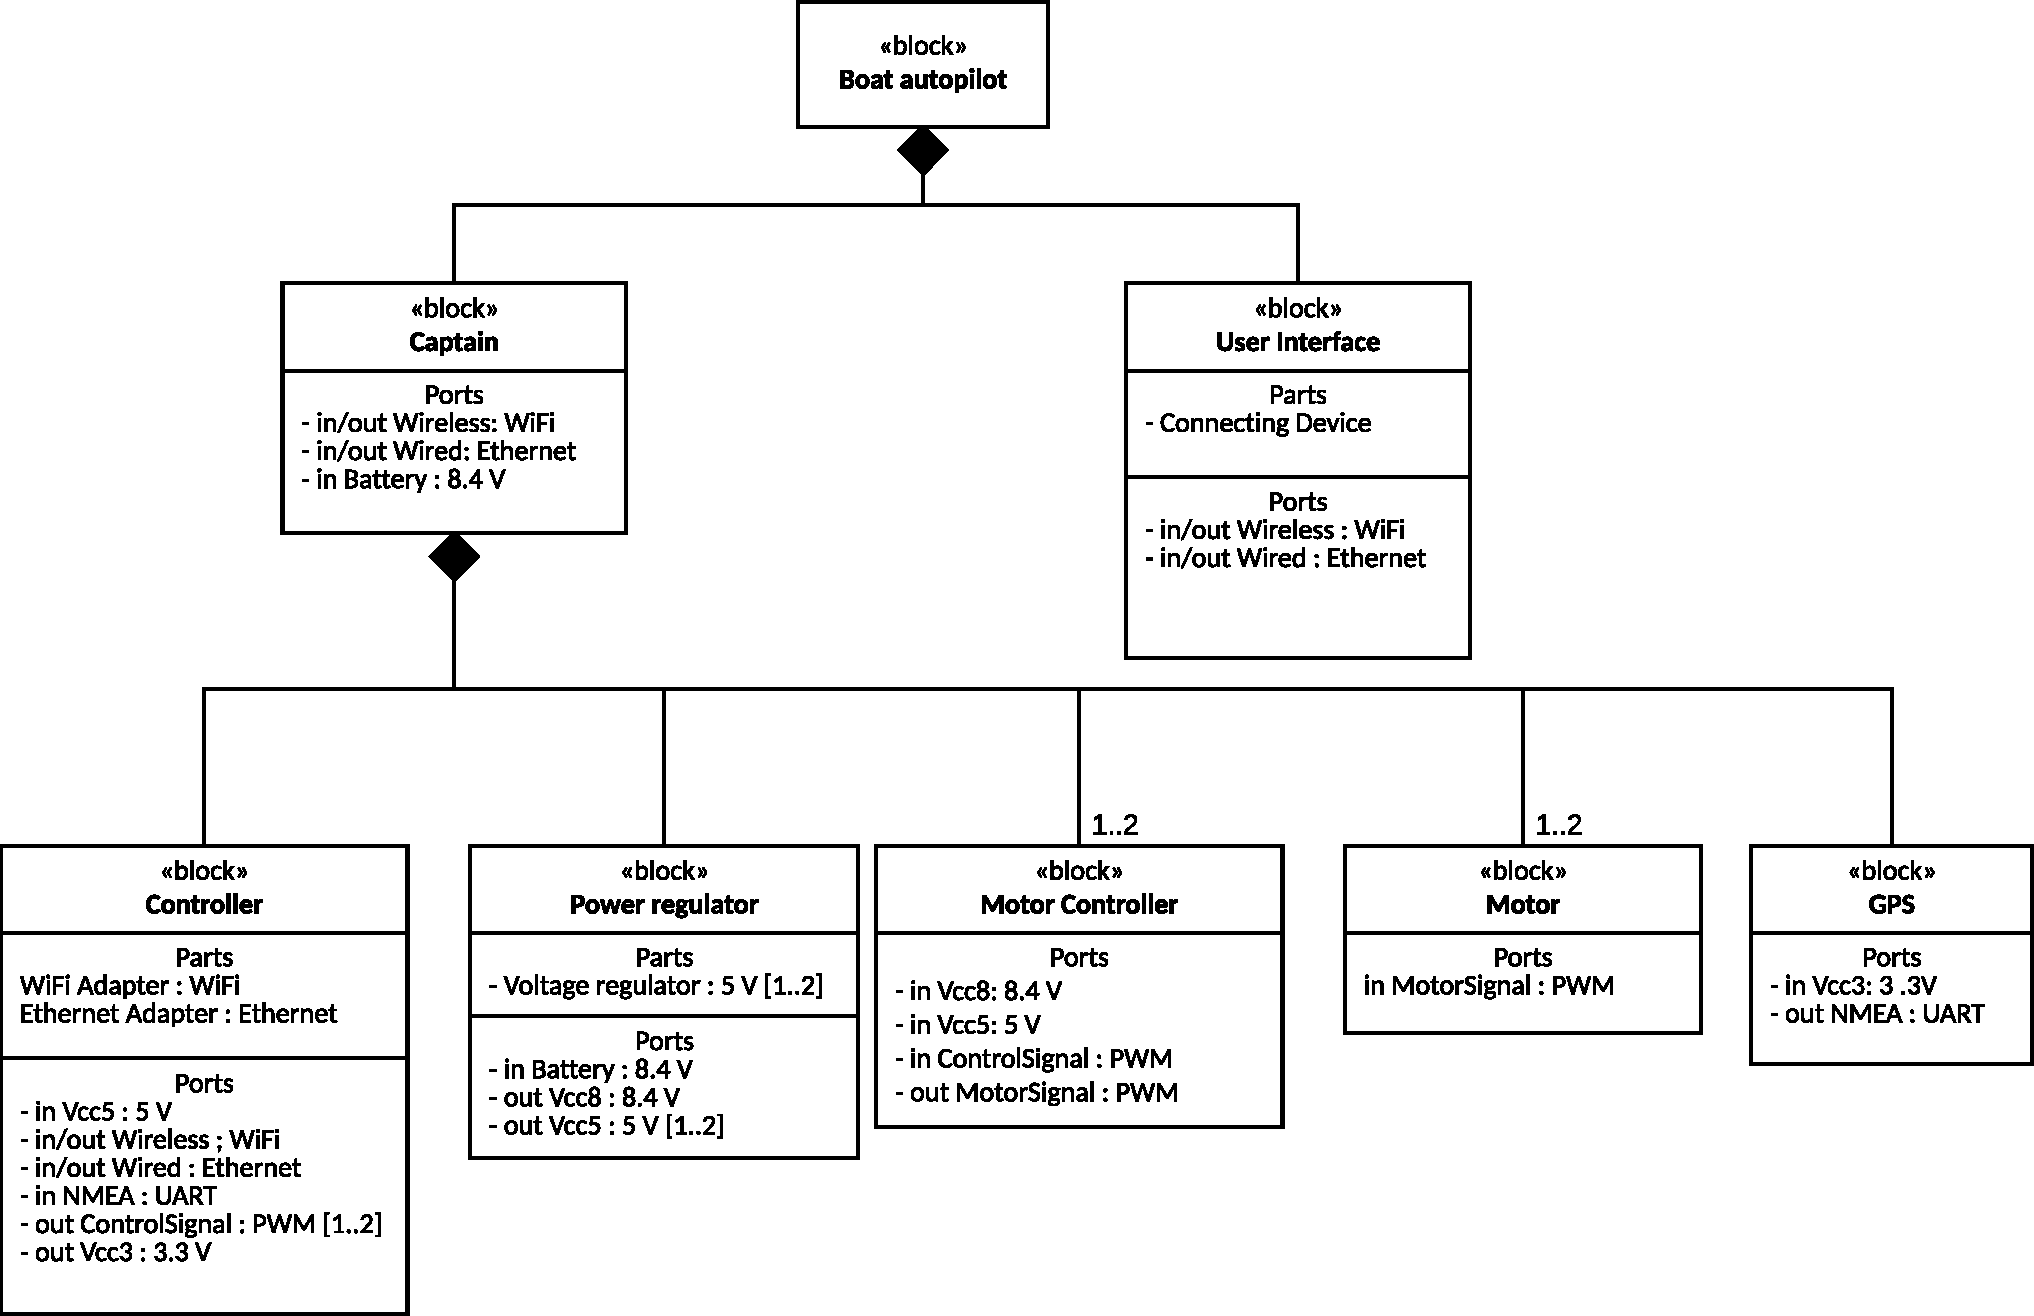
\includegraphics[width=1\linewidth]{../Appendix/Project/Dokumentation/Images/System_architecture/General_BDD}
\caption{General block definition diagram (BDD)}
\label{fig:generalbdd}
\end{figure}

The system can be broken down into two separate parts. One is the user interface, this is a clients personal computer. This personal computer needs to have either WiFi or an Ethernet port, this is so it can connect to the system. The system is the other part, and it has been named Captain. 

Captain is the hardware platform for this project, and it also needs WiFi and an Ethernet port, so it can be connected to. Further more it needs an external battery to power it.  Captain is also built up of subcomponents, or parts. these parts are; a GPS, 1 to 2 motors, 1 to 2 motor controllers, a power regulator, and a controller. The controller is the brain of the operation, it communicates with the user interface, and dictate what the motors should do, and it reads from the GPS receiver. The power regulator is used to regulate the battery voltage, so the controller, the motor, and the motor controller can use it. The motor controller is used to take the control signals from the controller, and drive the motor with them. 

With the block now defined, an IBD or internal block diagram can be created, and seen in figure~\ref{fig:generalibd}. This diagram describe how the different blocks of the BDD connect to each other, via the signals that are defined in the BDD as well. A full signal list and description can be found in the documentation in section~\ref{sec:general_ibd} on page~\pageref{sec:general_ibd}.
\begin{figure}[H]
\centering
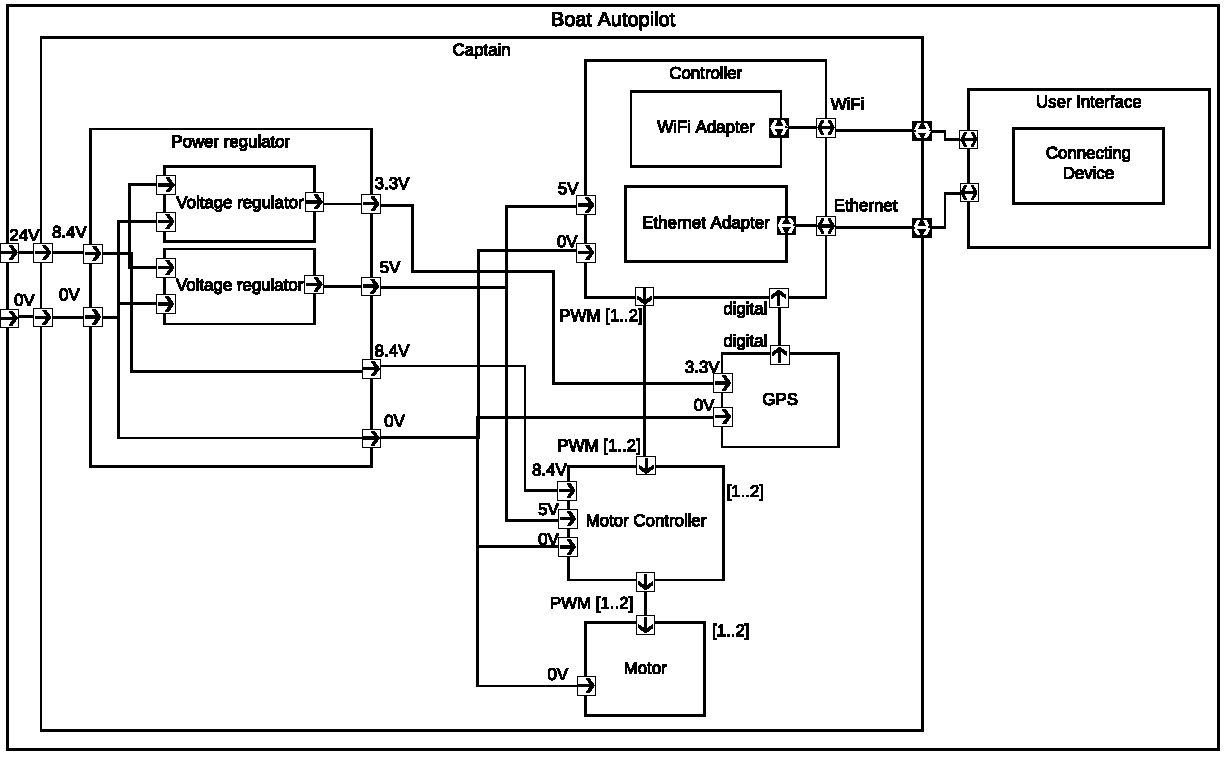
\includegraphics[width=1\linewidth]{../Appendix/Project/Dokumentation/Images/System_architecture/General_IBD}
\caption{General internal block diagram (IBD)}
\label{fig:generalibd}
\end{figure}

\section{Software architecture}
The software architecture is described with a domain model, an application model and several sequence diagrams. 

Lets start out by having a look at the domain model, it can be seen on figure~\ref{fig:domainmodel}. The domain model is used to describe the system should act to an actor interacting with it. In the domain model it can be seen how the user or technician can interact with the web interface, and how it then communicates to the controller. The controller acts on the motors, which in turn change the boats position. This that affects, what the GPS receiver reads, and this information is then passed on to the controller. The information 

\begin{figure}[H]
\centering
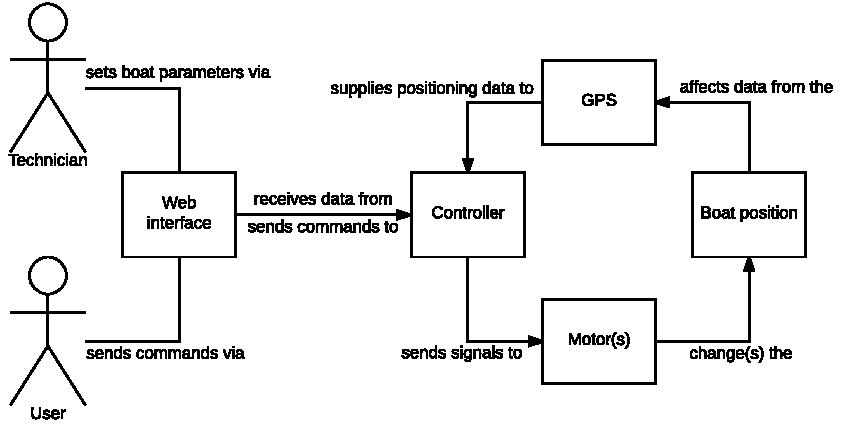
\includegraphics[width=1\linewidth]{../Appendix/Project/Dokumentation/Images/System_architecture/Domain_Model}
\caption{Domain model}
\label{fig:domainmodel}
\end{figure}

With a domain model and use cases, an application model can be created, as seen in figure~\ref{fig:applicationmodel}. It describes the functionality of the block from the domain model, it also classifies the blocks as either boundary, control or entity. A boundary block is something that interacts with the real world, a control block is the block that mediates functionality of boundary blocks and entity blocks. The entity block is a representation of information.

\begin{figure}[H]
\centering
\includegraphics[width=1\linewidth]{../Appendix/Project/Dokumentation/Images/System_architecture/Application_Model}
\caption{Application model}
\label{fig:applicationmodel}
\end{figure}

With the functionality of the blocks figured out in the application model, its time to look at sequence diagrams. There are a lot of sequence diagrams, so only a few interesting ones will be discussed in this report. For all the sequence diagrams, have a look in the documentation in section~\ref{sec:soft-architecture} on page~\pageref{sec:soft-architecture}.

The sequence diagrams follow the use cases, therefore lets have a look at the once that correspond to the once discussed in the requirements section, that is; use case 3 - "Edit parameter profile", use case 11 - "Calculate coverage path", use case 12 - "Run coverage path", and use case 5 - "Request diagnostics". 

Figure~\ref{fig:usecase3sd} explains how a technician edits a parameter. First the parameter profile is displayed, then it is edited by the technician.  

\begin{figure}[H]
\centering
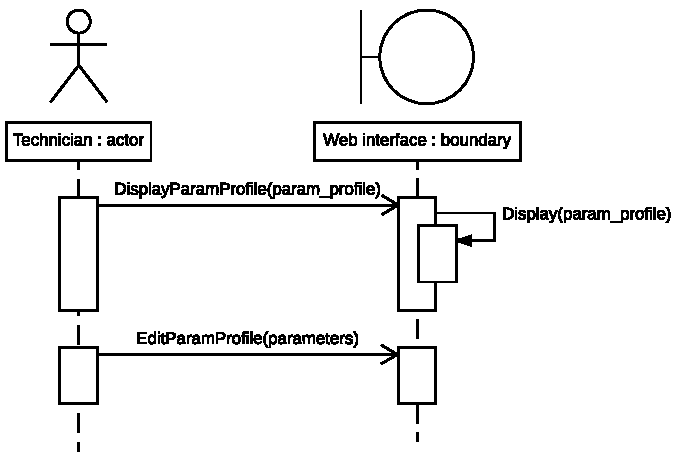
\includegraphics[width=1\linewidth]{../Appendix/Project/Dokumentation/Images/System_architecture/Use_case_3_SD}
\caption{Sequence diagram for use case 3 - "Edit parameter profile"}
\label{fig:usecase3sd}
\end{figure}

Figure~\ref{fig:usecase11sd} is showing how a user tells the system how to calculate a coverage path. This is done thought he user interface, which tells the controller to calculate a path. The controller uses GPS data to calculate the path and then returns the path to web interface. Then the path is displayed.

\begin{figure}[H]
\centering
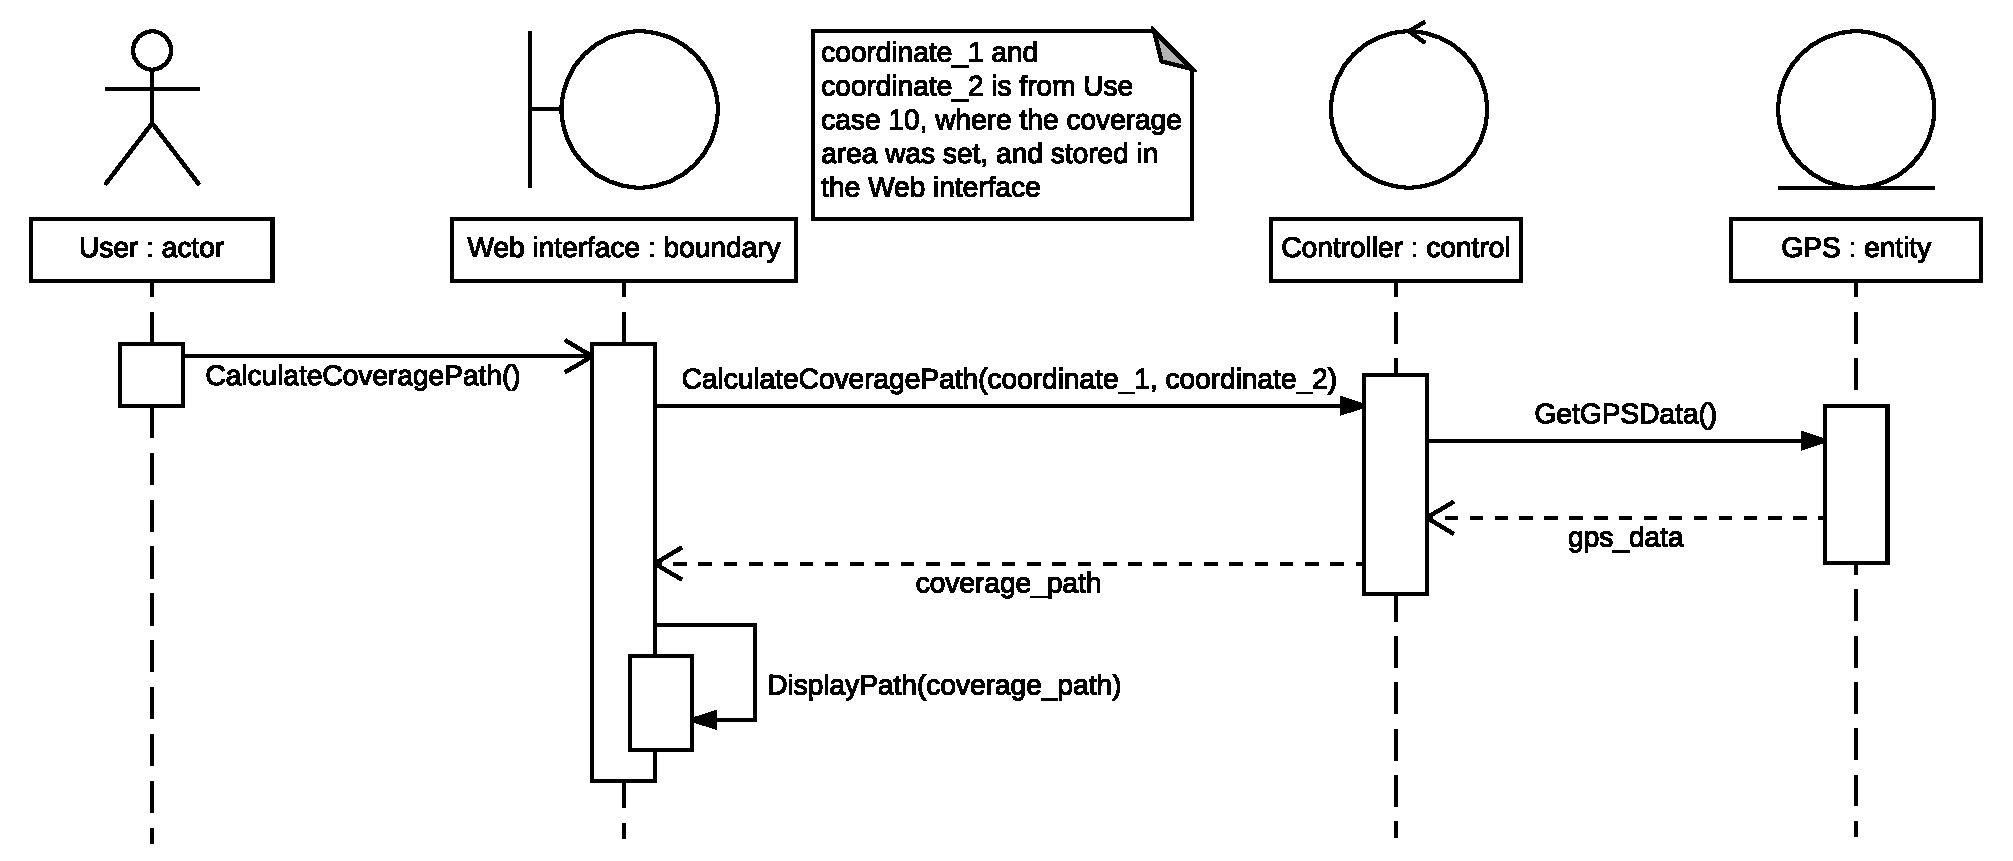
\includegraphics[width=1\linewidth]{../Appendix/Project/Dokumentation/Images/System_architecture/Use_case_11_SD}
\caption{Sequence diagram for use case 11 - "Calculate coverage path"}
\label{fig:usecase11sd}
\end{figure}

Figure~\ref{fig:usecase12sd} illustrates what happens in use case 12. When the user tells the web interface to run it relays the message to the controller which in turn starts a loop. This loop gets GPS data and tells the motors what to do. It tells the web interface to display the boat position. The controller also calculates the estimated time en-route and the web interface displays it.

\begin{figure}[H]
\centering
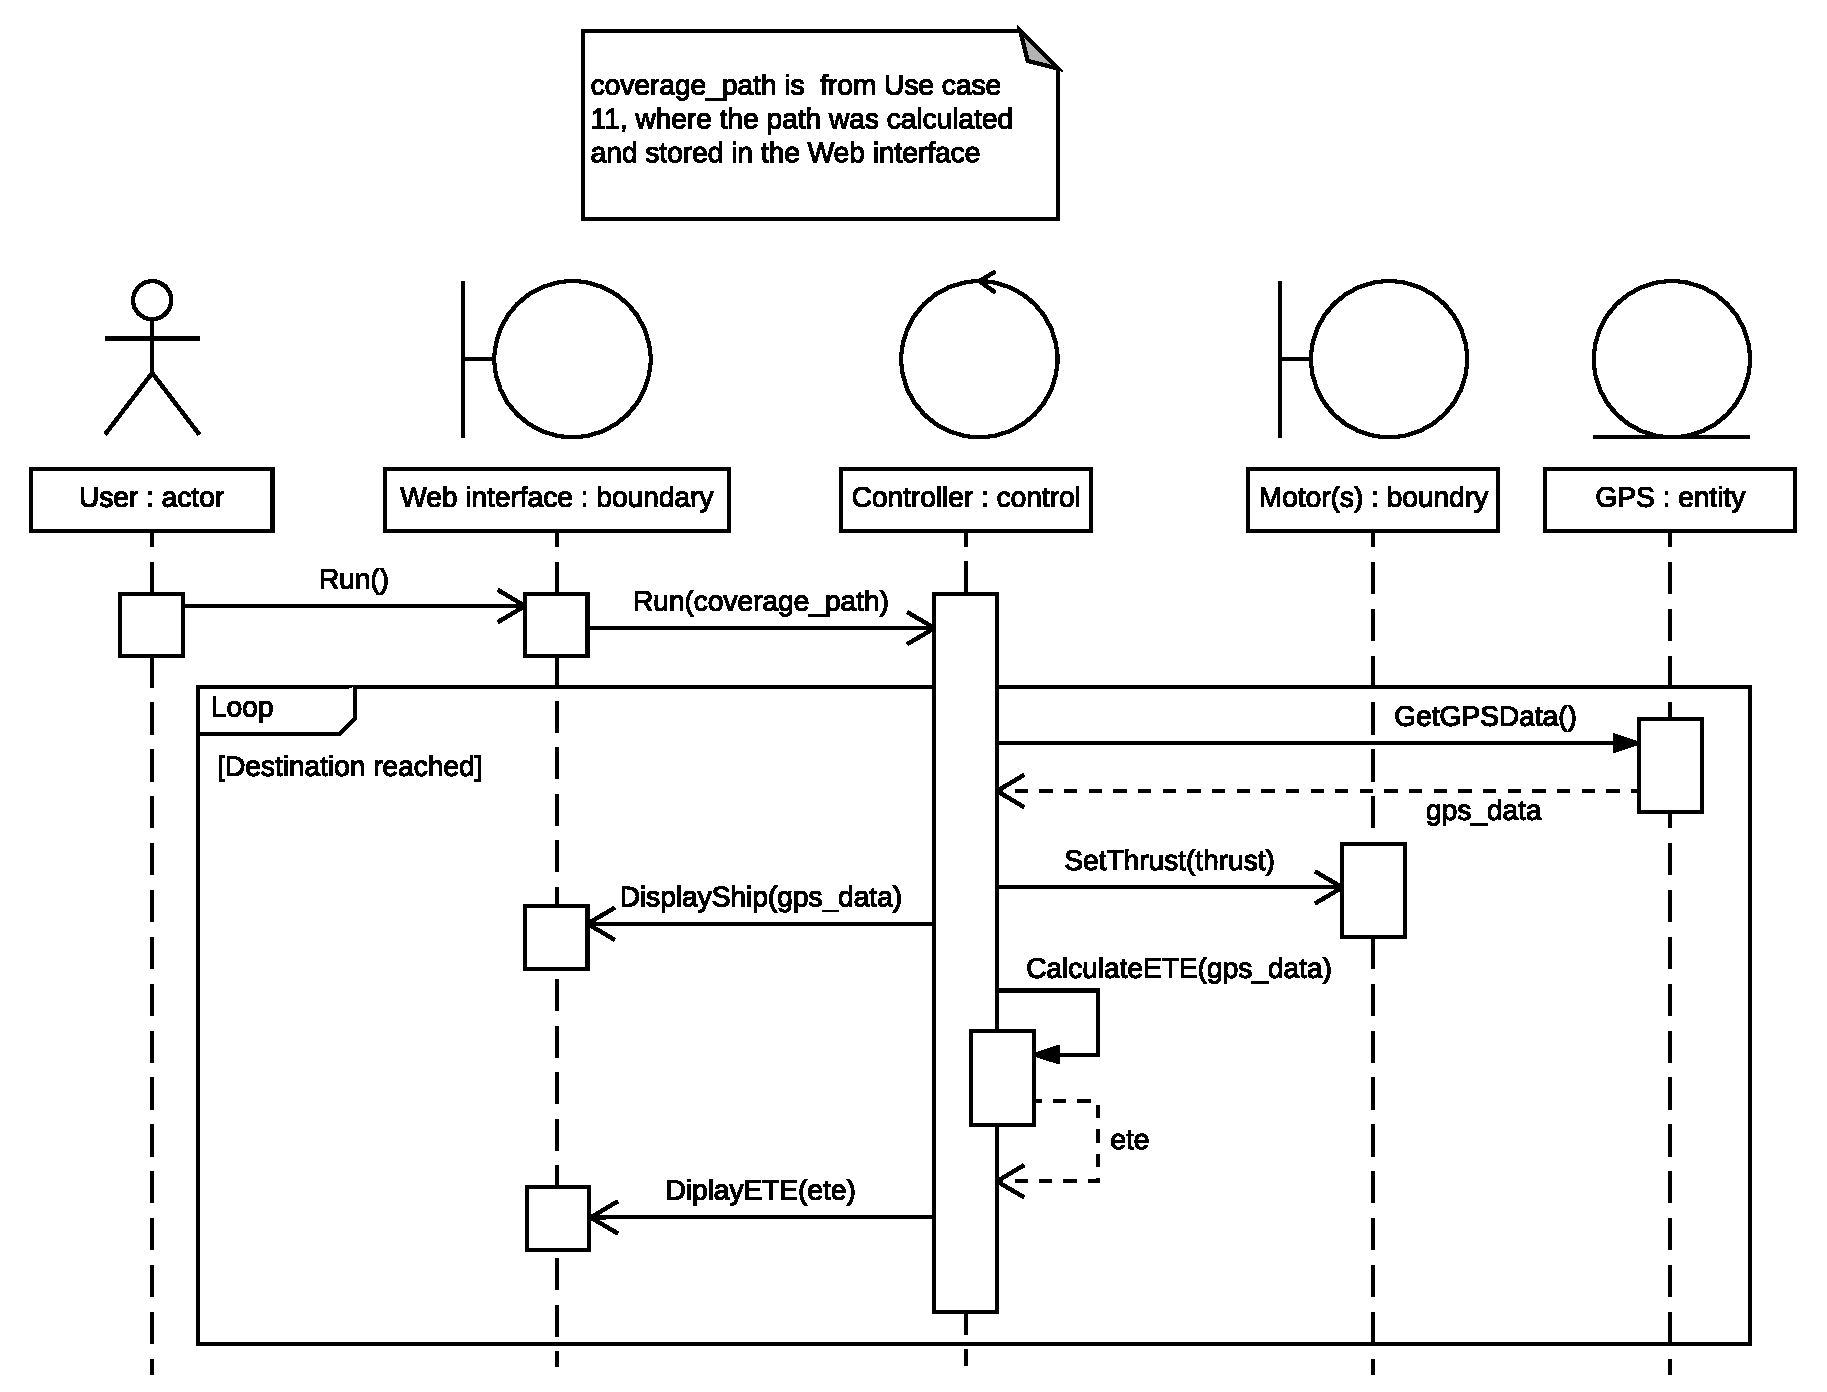
\includegraphics[width=1\linewidth]{../Appendix/Project/Dokumentation/Images/System_architecture/Use_case_12_SD}
\caption{Sequence digram for use case 12 - "Run coverage path"}
\label{fig:usecase12sd}
\end{figure}

Lastly, figure~\ref{fig:usecase5sd} show how the system get and displays diagnostics data. When the user requests diagnostics data, the web interface asks the controller for it. The controller responds by getting the current thrust of the motor and the GPS data along with the GPS diagnostics data. The controller also get connection diagnostics from the web interface, all of this is then displays on the web interface.

\begin{figure}[H]
\centering
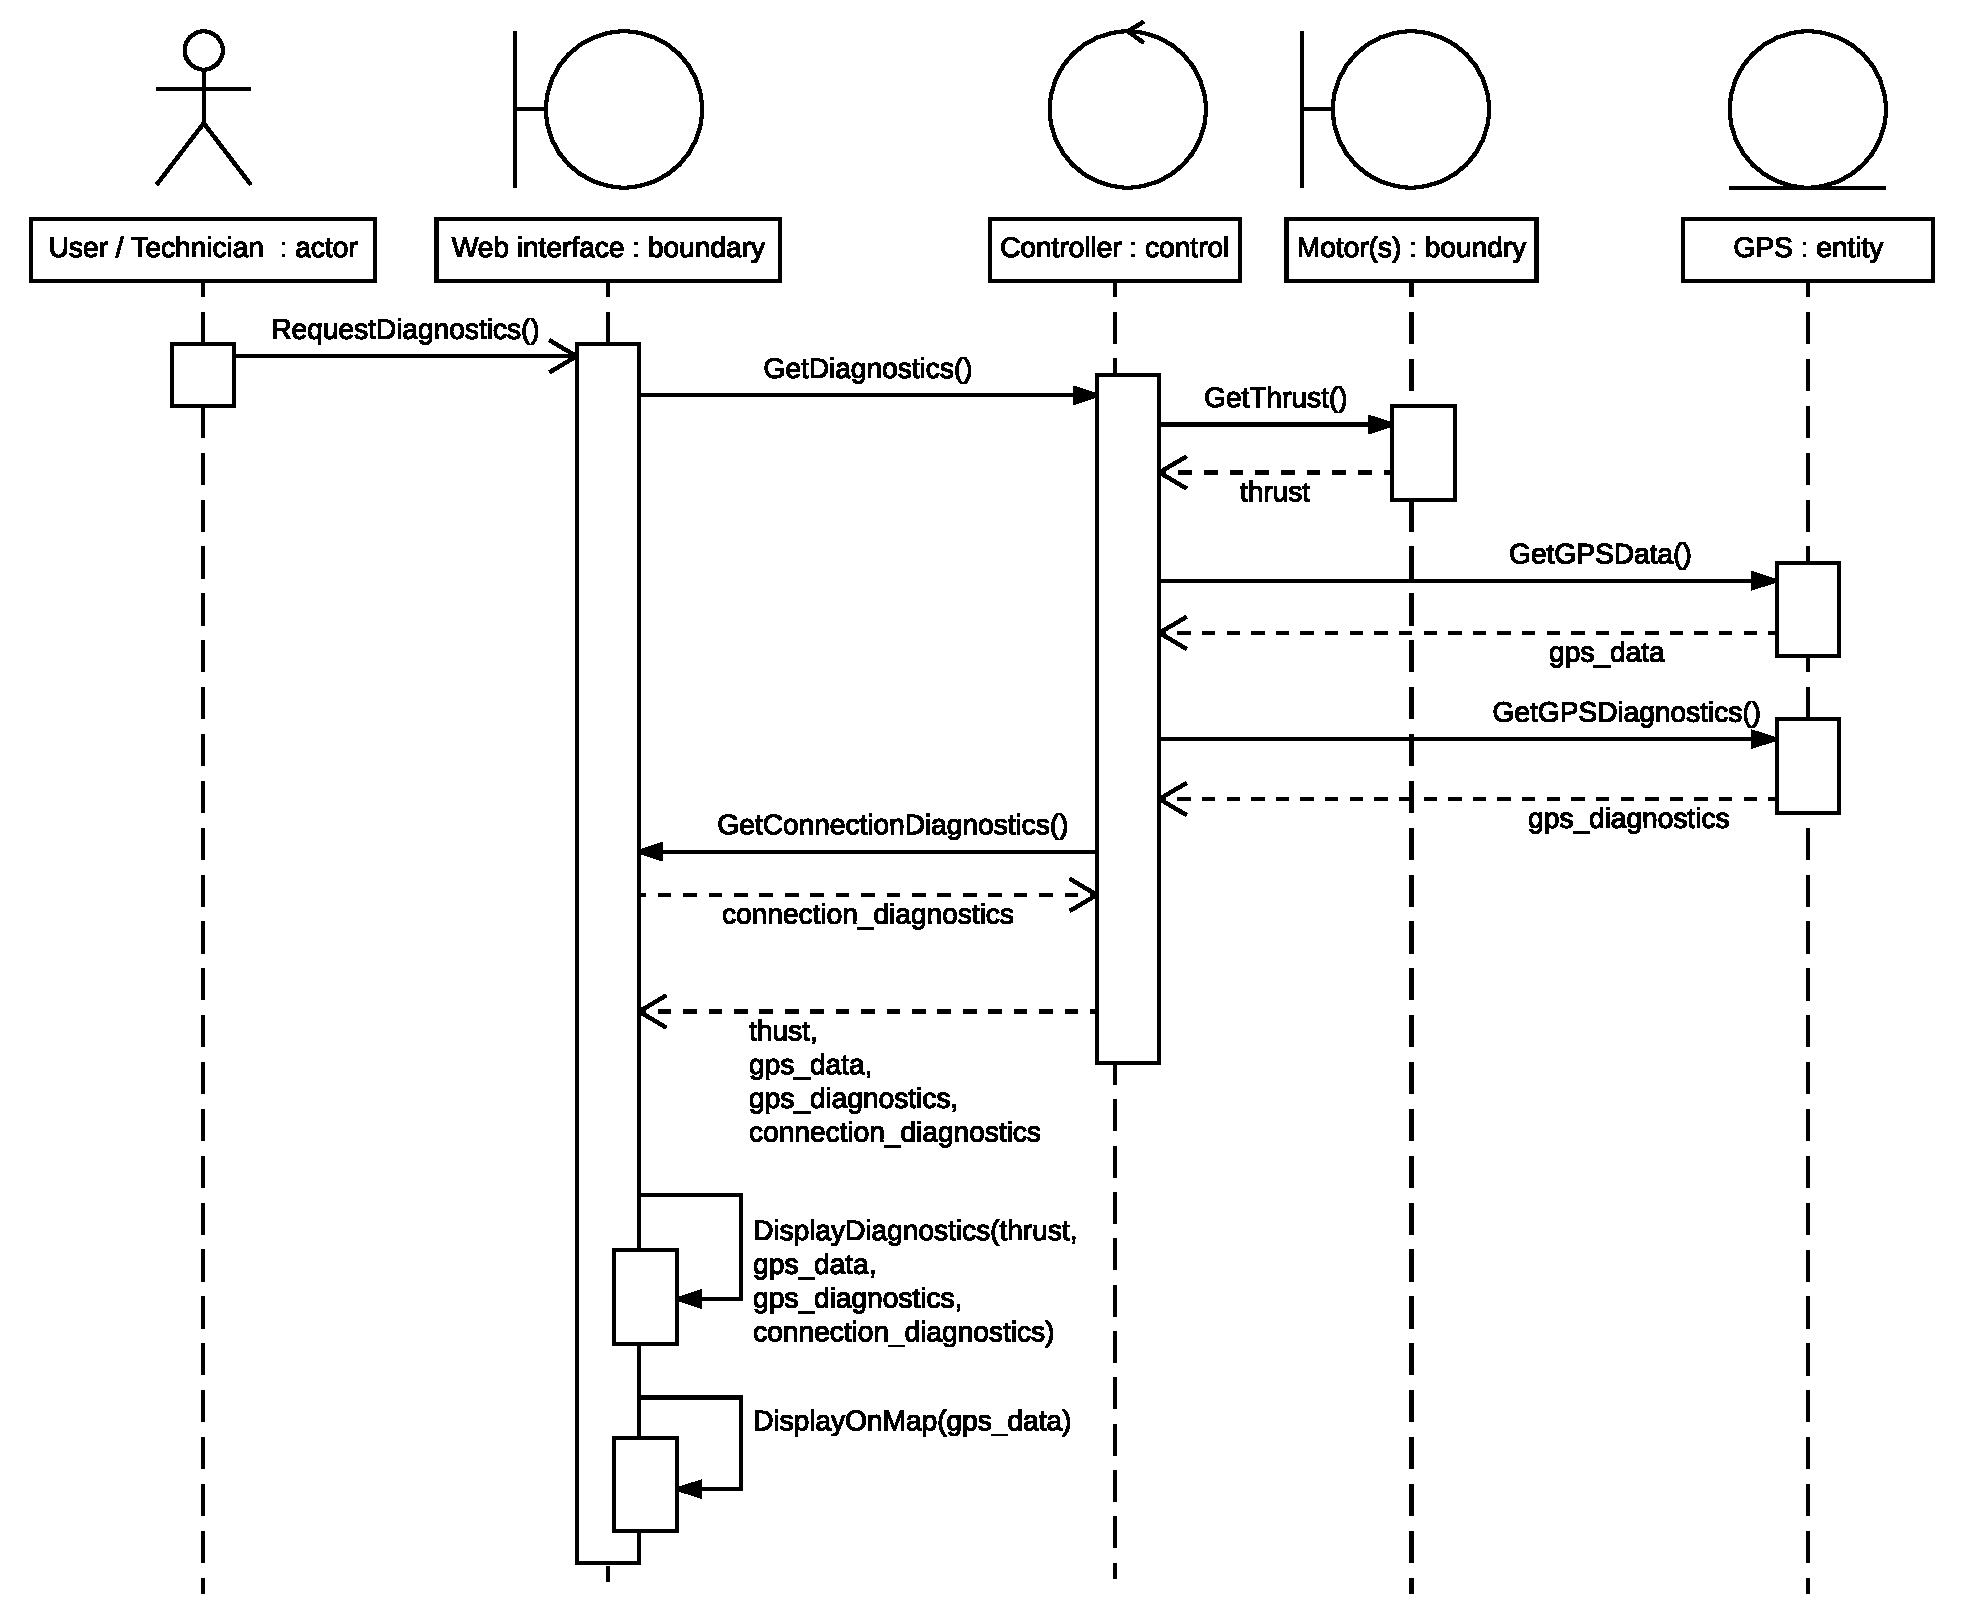
\includegraphics[width=1\linewidth]{../Appendix/Project/Dokumentation/Images/System_architecture/Use_case_5_SD}
\caption{Sequence diagram for use case 5 - "Request diagnostics"}
\label{fig:usecase5sd}
\end{figure}











